\section{The ForeC Language}
\label{sec:forecLanguage}

%-----------------------------------------------------------------------------

\subsection{The Synchronous Approach}
Synchronous languages are based on the synchrony hypothesis~\cite{timed_synchronous_survey},
which states that a system reacts instantaneously to new environmental
inputs. Thus, the synchrony hypothesis assumes that the system 
executes infinitely fast, i.e., in zero time. This separates the physical 
time of the environment from the execution time of the implemented system. 
Figure~\ref{fig:synchronous_moc} depicts a synchronous 
program, defined as a set of concurrent threads, interacting with the 
environment. Synchronous programs are driven by a hypothetical (logical)
\emph{global clock} that triggers the execution of the program. The speed 
of the global clock is determined by the system's specifications. At each
global tick, the threads sample the environment, perform their computations,
and then emit their results to the environment. When a thread completes 
its computation, we say that the thread has completed its \emph{local tick}.
When all threads have completed their local tick, we say that the program
has completed its \emph{global tick}.
Concurrent threads can communicate with each other (dashed 
arrows in Figure~\ref{fig:synchronous_moc}) during their
computation. The communication is instantaneous due to 
the synchrony hypothesis.   
The separation of physical and execution time simplifies 
the language semantics and enables formal verification. Once the 
system is implemented, it is necessary to verify the synchrony 
hypothesis. That is, the Worst-Case Execution Time (WCET) of each 
global tick must not exceed the minimal inter-arrival time of inputs
from the environment.

\begin{figure}
	\centering
	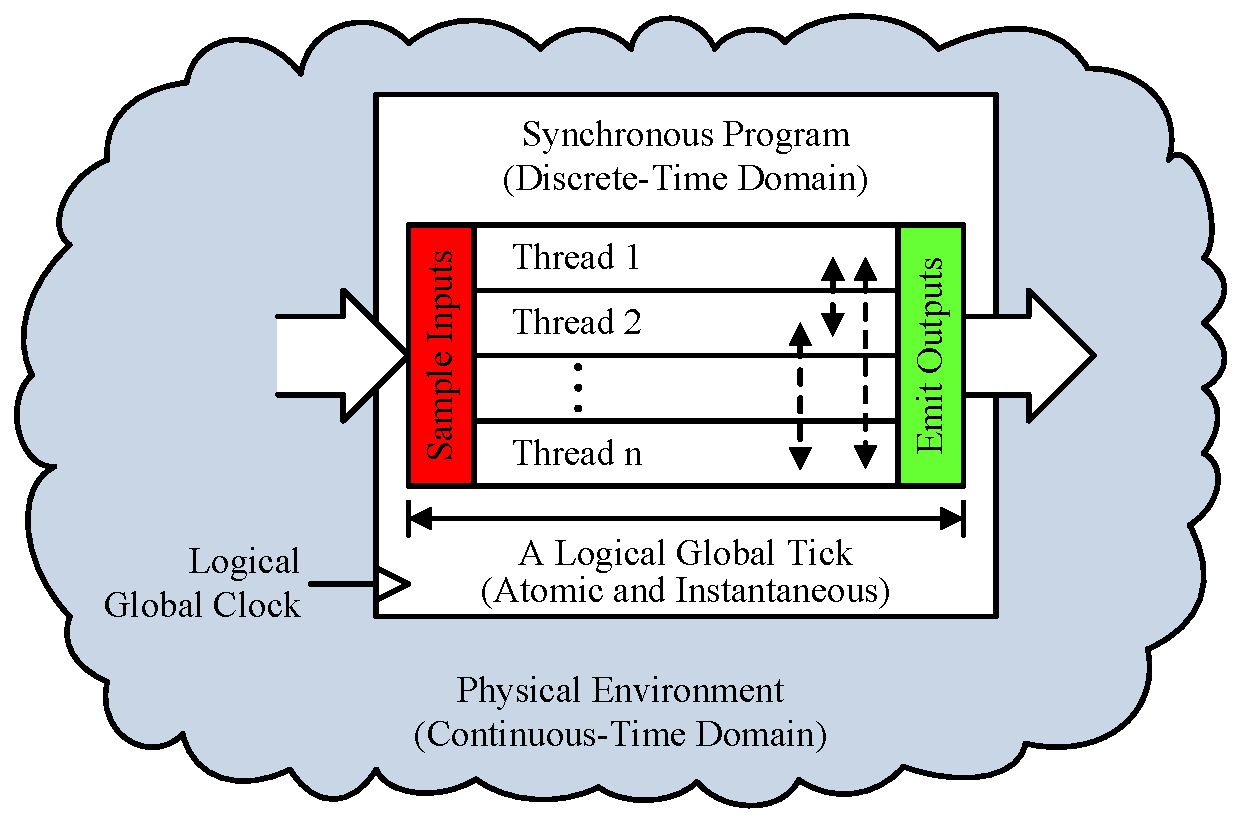
\includegraphics[width=0.6\columnwidth]{synchronous_moc}	

	\caption{Synchronous model of computation.}
	\label{fig:synchronous_moc}
\end{figure}

ForeC extends the C language with synchronous constructs to 
enable the deterministic parallel programming of multicores.
Extending C with synchronous constructs is not new, as the 
following languages demonstrate: Esterel-C Language (ECL~\cite{timed_ecl}), 
\synchronousc{} (SC~\cite{timed_synccharts_c_proposal}), Reactive 
Shared Variables~\cite{timed_reactivec_shared_variables}, 
and \pretc{}~\cite{pret_pretc}. The ECL compiler splits an 
ECL program into an Esterel and a C program. The Esterel program
is compiled in the traditional manner~\cite{timed_compiling_esterel}, 
where the concurrency is compiled away and, therefore, unsuitable for multicore execution.
The inherent sequential execution semantics of SC, Reactive C 
and \pretc{} renders them unsuitable for multicore execution. In
contrast, ForeC is designed for parallel execution and parallel 
threads can be scheduled to execute in arbitrary order without 
altering the program's behavior. This scheduling 
independence is maintained even when threads communicate using 
shared variables. Thus, a range of scheduling strategies can be 
used to achieve time-predictable implementations without sacrificing
much throughput. The remainder of this section details the 
syntax and semantics of the ForeC synchronous constructs.


%-----------------------------------------------------------------------------

\subsection{The ForeC Language Constructs}
ForeC extends a subset of C (see
Section~\ref{sec:forecLanguage_programming}) with a minimal
set of statements and type qualifiers.
Figure~\ref{fig:forec_syntax} gives the extended syntax and
Table~\ref{table:forec_semantics} summarizes the semantics.
A statement (\emph{st}) in ForeC is a traditional C
statement or block within \verb${$ and \verb$}$
(\emph{c\_st}), barrier statement (\verb$pause$), fork/join
(\verb$par$), or preemption (\verb$abort$). Like C, extra
properties can be specified for variables using type
qualifiers. A type qualifier (\emph{tq}) in ForeC is a
traditional C type qualifier (\emph{c\_tq}), an environment
interface variable (\verb$input$ and \verb$output$), or
shared variable amongst threads (\verb$shared$). The ForeC
type qualifiers precede the C type qualifiers in variable
declarations. 

We use a simple ForeC program called
\verb$UAV$ in Figure~\ref{fig:forec_uav} to elucidate the
semantics of the language. \verb$UAV$ controls an unmanned
aerial vehicle and Figure~\ref{fig:forec_uav_tasks}
illustrates its functionality as a block diagram of
tasks. The \verb$Nav$ task localizes the UAV using on-board
sensors, updates the flight path, and sends the desired
position to the \verb$Stability$ task. The \verb$Stability$
task controls the flight surfaces to ensure stable flight to
the desired position. Extremely low jitter is required for
stable flight. The \verb$Avoid$ task uses on-board sensors
to detect obstacles around the UAV and sends collision
avoidance data to the \verb$Nav$ task. Thus, the more
frequent obstacles are checked for, the faster the UAV can
safely travel at. To help illustrate \verb$UAV$'s execution
behavior, Figure~\ref{fig:forec_uav_timing1} shows a
possible execution trace.

\begin{figure}[t]
	\centering

	\renewcommand{\arraystretch}{1.25}
	\begin{tabular}{l r l}
		Statements:			& \emph{st} & ::= \emph{c\_st} | \verb$pause$ | \verb$par($\emph{st},~\emph{st}\verb$)$	\\
							&			& ~~~| \verb$weak$?~\verb$abort$~\emph{st}~\verb$when immediate$?~(\expression{})		\\
																																\\
		Type Qualifiers:	& \emph{tq}	& ::= \emph{c\_tq} | \verb$input$ | \verb$output$ | \verb$shared$
	\end{tabular}
	
	\caption{The syntactic extensions to C.}
	\label{fig:forec_syntax}
\end{figure}

\begin{table}[t]
	\centering
	\renewcommand{\arraystretch}{1.25}		

	\begin{tabular}{| p{\textwidth} |}
		\hline
		\textbf{ForeC construct and its Semantics}										\\ 
		\hline
		\verb$input$:
			Type qualifier to declare an input variable, the value of which is updated 
			by the environment at the start of every global tick.						\\ \hline
		\verb$output$:
			Type qualifier to declare an output variable, the value of which is emitted 
			to the environment at the end of every global tick.							\\ \hline
		\verb$shared$:
			Type qualifier to declare a shared variable, which can be accessed by 
			multiple threads.															\\ \hline
		\verb$pause$:
			Pauses the executing thread until the next global tick.						\\ \hline
		\verb$par$(\emph{st},\emph{st}):
			Forks two statements \emph{st} as parallel threads. The 
			\verb$par$ terminates when both threads terminate (join back).				\\ \hline
		\verb$weak$?~\verb$abort$~\emph{st}~\verb$when immediate$?~(\expression{}):
			Preempts its body \emph{st} when the expression \expression{} evaluates to 
			a non-zero value. The optional \verb$weak$ and \verb$immediate$ keywords 
			modify its temporal behavior.												\\
		\hline
	\end{tabular}

	\caption{Semantics of the ForeC constructs.}
	\label{table:forec_semantics}
\end{table}

\begin{figure}
	\centering

	\begin{minipage}[t]{0.75\columnwidth}
		\lstinputlisting[style=full]{./code/uav.forec}
	\end{minipage}

	\caption{\texttt{UAV}, an example ForeC program.}
	\label{fig:forec_uav}
\end{figure}

\begin{figure}
	\centering

	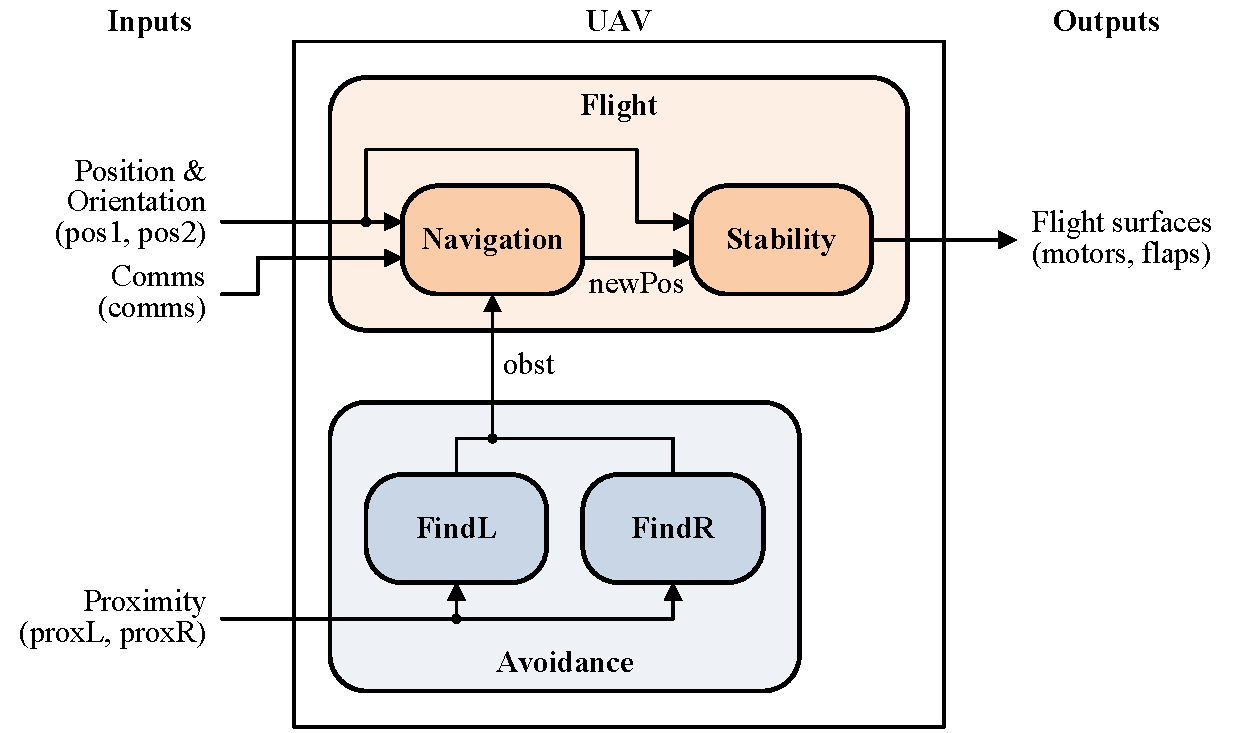
\includegraphics[width=\columnwidth]{images/uav_tasks.pdf}

	\caption{Tasks of \texttt{UAV}.}
	\label{fig:forec_uav_tasks}
\end{figure}

\begin{figure}
	\centering

	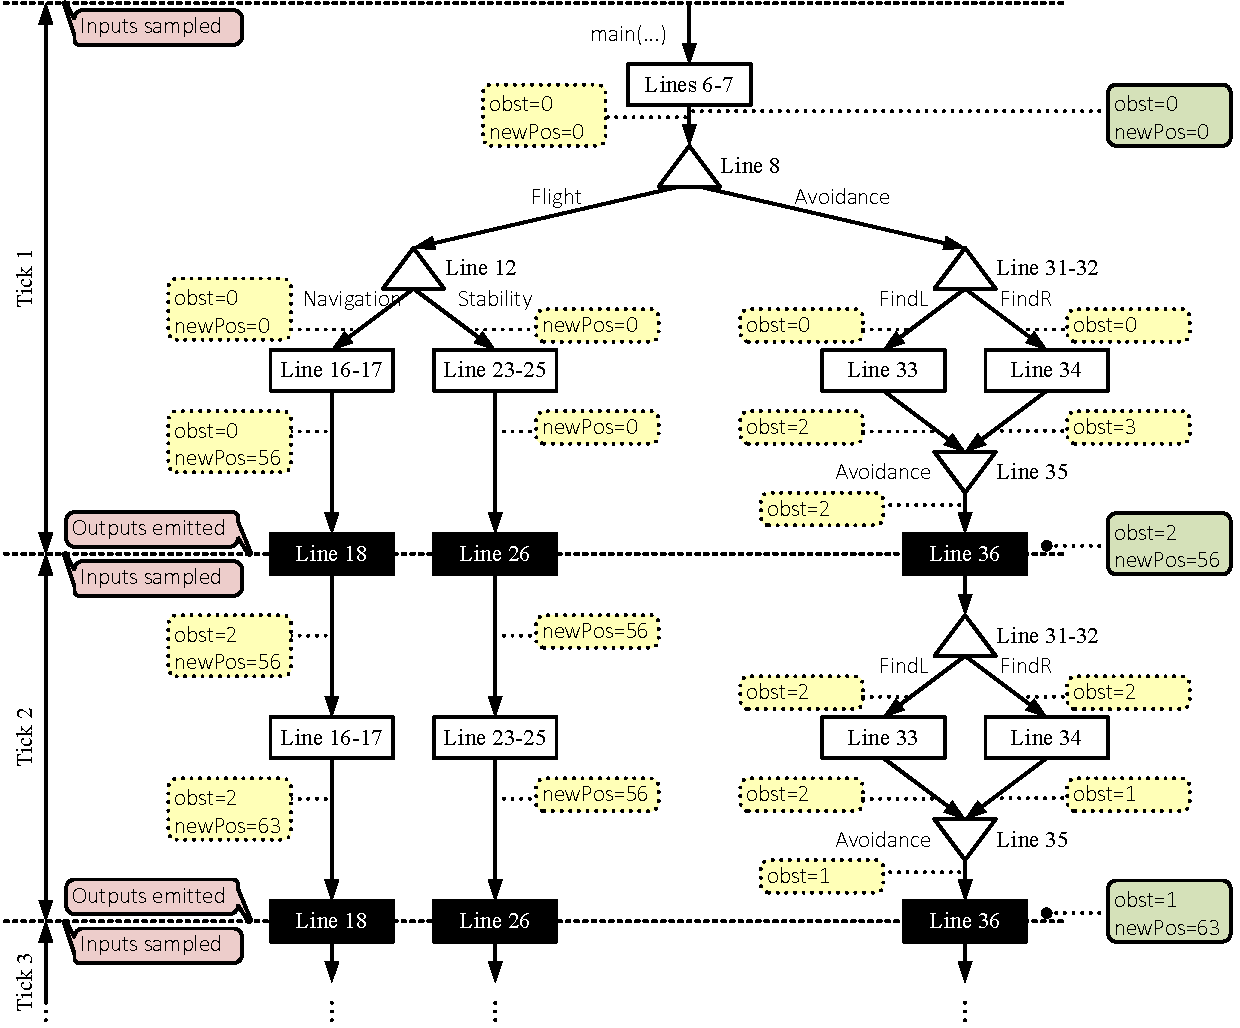
\includegraphics[width=\columnwidth]{images/uav_timing1.pdf}

	\caption{Possible execution trace of \texttt{UAV}.}
	\label{fig:forec_uav_timing1}
\end{figure}

\begin{figure}
	\centering

	\subfloat[Thread hierarchy.] {
		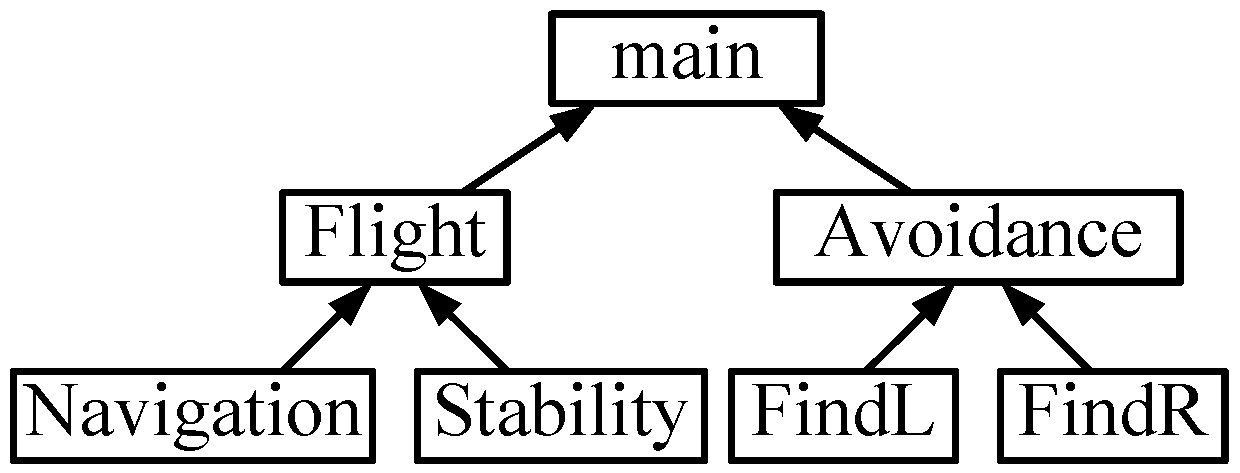
\includegraphics[width=0.35\columnwidth]{uav_genealogy_hierarchy}
		\label{fig:forec_uav_genealogy_hierarchy}
	}
	\subfloat[Thread genealogy examples.] {
		\begin{minipage}[b]{0.6\textwidth}
			\small
			\begin{itemize}
				\item \texttt{main} is the parent of \texttt{Flight} and \texttt{Avoid}. 
					  \texttt{Flight} is the parent of \texttt{Nav} and \texttt{Stability}.

				\item \texttt{main} and \texttt{Flight} are ancestors of \texttt{Nav} and \texttt{Stability}.
				
				\item \texttt{FindL} and \texttt{FindR} are siblings.
				
				\item \texttt{Nav} is a relative of \texttt{Stability}, \texttt{Avoid}, \texttt{FindL}, and \texttt{FindR}.
			\end{itemize}
		\end{minipage}
		\label{fig:forec_uav_genealogy_description}
	}
	
	\caption{Thread genealogy of \texttt{UAV}.}
	\label{fig:forec_uav_genealogy}
\end{figure}


%-----------------------------------------------------------------------------

\subsection{Interface with the Environment}
\label{sec:forecLanguage_io}
The \verb$UAV$ program begins with the inclusion of a C header file 
(line~\ref{code:forec_uav_header}) for the functions used in the 
program and global variable declarations 
(lines~\ref{code:forec_uav_inputs}-\ref{code:forec_uav_outputs}) to 
interface with the environment. Line~\ref{code:forec_uav_inputs}
declares input variables to capture sensor readings. Input 
variables are read-only and their values are 
updated by the environment at the start of every global tick. 
Line~\ref{code:forec_uav_outputs} declares output variables to
hold actuation commands for the flight motors and surfaces.
Output variables emit their values to the environment at 
the end of every global tick. Input and output variables can only be 
declared in the program's global scope.


%-----------------------------------------------------------------------------

\subsection{Fork/Join Parallelism}
Like traditional C programs, the \verb$main$ function 
(line~\ref{code:forec_uav_main}) is the main 
entry point of \verb$UAV$ and serves as the initial
thread of execution. Lines~\ref{code:forec_uav_obst}-\ref{code:forec_uav_newpos}
declare variables that can be shared among multiple 
threads (see Section~\ref{sec:forec_shared_variables}).
In Figure~\ref{fig:forec_uav_timing1}, the states of 
the shared variables are given inside solid round
boxes at specific points in the execution trace.
Line~\ref{code:forec_uav_obst} uses the \verb$Obst$ C-struct
(line~\ref{code:forec_uav_struct}) to declare a shared
variable \verb$obst$ for storing the distance (\verb$d$) and
angle (\verb$a$) to the closest obstacle found.
Line~\ref{code:forec_uav_newpos} declares a shared variable
\verb$newPos$ to store the UAV's desired position. 

On line~\ref{code:forec_uav_par1}, the \verb$par$ statement
forks the \verb$Flight$ (line~\ref{code:forec_uav_flight})
and \verb$Avoid$ (line~\ref{code:forec_uav_avoid}) functions
into two parallel child threads. We name the threads by
their function names, e.g., threads \verb$Flight$ and
\verb$Avoid$. The \verb$Flight$ thread forks two more
parallel child threads, \verb$Nav$
(line~\ref{code:forec_uav_nav}) and \verb$Stability$
(line~\ref{code:forec_uav_stability}), creating a nesting
(hierarchy) of threads. The threads \verb$Nav$,
\verb$Stability$ and \verb$Avoid$ implement the three tasks
in Figure~\ref{fig:forec_uav_tasks}. The \verb$par$ can also
fork blocks of code, e.g., line~\ref{code:forec_uav_par3}.
The \emph{parent} thread is also the \emph{ancestor} of its 
child threads and their nested child threads.
Child threads forked by the same
\verb$par$ are \emph{siblings}. The \verb$par$ is
a blocking statement and terminates only when both its child
threads have terminated. Consequently, threads always
execute sequentially with respect to their ancestors.
Threads that are not ancestors of each other are
\emph{relatives} and can execute in parallel. The thread
genealogy of a program can be determined statically by
inspecting the program's control-flow.
Figure~\ref{fig:forec_uav_genealogy_hierarchy} shows the
thread hierarchy of the \verb$UAV$ program. Each node is a
thread and arrows are drawn from the child threads to their
parent. Figure~\ref{fig:forec_uav_genealogy_description}
exemplifies the thread genealogy.


%-----------------------------------------------------------------------------

\subsection{Barrier Synchronisation}
After the \verb$Nav$, \verb$Stability$, and \verb$Avoid$
threads have forked, they start executing their bodies.
The \verb$Nav$ thread, for example, enters the \verb$while$
loop (line~\ref{code:forec_uav_while1}) and computes a new
desired position (line~\ref{code:forec_uav_plan}). Next, the
\verb$pause$ statement pauses the thread's execution 
(line~\ref{code:forec_uav_pause1}), acting as a
synchronization barrier. We say that a thread completes its
\emph{local tick} when it pauses, terminates, or forks at
least one thread that completes their local tick without
terminating. For example, when the \verb$Avoid$ thread is 
forked, it starts its first local tick (line~\ref{code:forec_uav_while2}) 
by forking the child threads \verb$FindL$ and \verb$FindR$ 
(line~\ref{code:forec_uav_par3}). Assuming that the \verb$find$ 
function does not pause, both child threads complete their 
local tick by terminating. After the child threads join, 
the \verb$Avoid$ thread reaches a \verb$pause$ (line~\ref{code:forec_uav_pause2})
and completes its first local tick.
The program completes its \emph{global tick}
when all threads have completed their respective local tick. At the
next global tick, the paused threads begin their
next local tick from their respective \verb$pause$. 
For brevity, we shorten the phrase \emph{global
tick} to the word \emph{tick} and use the phrase \emph{local
tick} as before.


%-----------------------------------------------------------------------------

\subsection{Shared Variables}
\label{sec:forec_shared_variables}
All variables in ForeC follow the scoping rules of C. By
default, all variables are \emph{private} and can only be
accessed (read or write) by one thread throughout its scope.
To allow a variable to be accessed by multiple threads, it
must be declared as a \emph{shared} variable using the
\verb$shared$ type qualifier. Thus, shared variables are
easy to identify and any misuse of private variables are
easy to detect at compile time. ForeC defines the semantics
of shared variables for thread-safe sharing without needing
to use mutual exclusion constructs. The goal is to provide
deterministic shared variable semantics that is agnostic to
scheduling. This goal is essential for the reasoning and
debugging of parallel programs. Within each tick, accesses
to a shared variable may occur in sequence or in parallel to
each other. Below and in
Table~\ref{table:forec_variable_access}, we define when
accesses are in sequence or in parallel to each other:

\begin{definition}
	\label{def:forec_access_sequential}
	Sequential access: Accesses from two threads are in sequence if both 
	threads are not relatives, or the accesses occur in different ticks. 
\end{definition}

\begin{definition}
	\label{def:forec_access_parallel}
	Parallel access: Accesses from two threads are in parallel if both 
	threads are relatives and the accesses occur in the same tick.
\end{definition}

\begin{table}[t]
	\centering
	\renewcommand{\arraystretch}{1.25}		

	\begin{tabular}{| c | c | c | c |}
		\cline{3-4}
		\multicolumn{1}{c}{}																& 				& \multicolumn{2}{| p{5cm} |}{\textbf{Accesses to the shared variable are by relative threads?}}	\\ 
		\cline{3-4}
		\multicolumn{1}{c}{}																& 				& \textbf{Yes}		& \textbf{No}																	\\ \cline{1-4}
		\multirow{2}{5.5cm}{\textbf{Accesses to the shared variable are in the same tick?}}	& \textbf{Yes}	& Parallel Access	&																				\\ \cline{2-3} 
																							& \textbf{No}	& \multicolumn{2}{c|}{Sequential Access}															\\
		\hline
	\end{tabular}

	\caption{Determining whether two accesses to a shared variable are parallel or sequential.}
	\label{table:forec_variable_access}
\end{table}

\begin{table}[t]
	\centering
	\renewcommand{\arraystretch}{1.25}		

	\begin{tabular}{| p{\textwidth} |}
		\hline
		\textbf{Programming Constructs:}
		These are constructs written in the host language to provide mechanisms for the 
		programmer to achieve mutual exclusion. Examples include: locks, mutex, semaphores, monitors, 
		transactional memory, message passing, and parallel data structures. Using these 
		constructs correctly can be tedious and error prone for large programs and may lead to other 
		errors~\cite{multiprocessing_problem_threads,multiprocessing_debugging_concurrency,multiprocessing_debugging_concurrency_study}, 
		e.g, deadlocks, starvation, or priority inversion.									\\ \hline
		
		\textbf{Language Semantics:}
		The language semantics ensures that race conditions are not possible. However, the 
		resulting memory model may only be suitable to a few types of applications. Examples include: synchronous 
		languages~\cite{timed_synchronous_survey}, \pretc{}~\cite{pret_pretc}, SharC~\cite{multiprocessing_sharc}, 
		Deterministic Parallel Java~\cite{multiprocessing_dpj}, SHIM~\cite{multiprocessing_shim_cell}, 
		SigmaC~\cite{multiprocessing_sigmac}, Concurrent Revisions~\cite{BurckhardtL11}, 
		Reactive Shared Variables~\cite{timed_reactivec_shared_variables}, and Synchronous 
		C~\cite{timed_synccharts_c_proposal}. 												\\ \hline
		
		\textbf{Static Analysis:}
		A compiler or static analyzer identifies and alerts the programmer regarding the race 
		conditions in their program (e.g., Parallel Lint~\cite{parallel_lint}) and may try 
		to resolve them by serializing the parallel accesses for the programmer 
		(e.g., Sequentially Constructive Concurrency~\cite{timed_seq_concurrency}). However, 
		programmer guidance is needed for race conditions that cannot be resolved.			\\ \hline
		
		\textbf{Runtime Support:}
		Programs are executed on a runtime layer that enforces deterministic execution 
		and memory accesses. 
		Examples include: CoreDet~\cite{multiprocessing_coredet}, Dthreads~\cite{multiprocessing_dthreads}, 
		Kendo~\cite{multiprocessing_kendo}, dOS~\cite{multiprocessing_dos}, Grace~\cite{multiprocessing_grace}, 
		DetMP~\cite{multiprocessing_detmp}, and DOMP~\cite{multiprocessing_domp}. Although repeated 
		executions of the same program are deterministic, the execution behavior is only 
		revealed at runtime.																\\ \hline
		
		\textbf{Hardware Support:}
		Parallel accesses are automatically detected and resolved by the hardware, preventing
		race conditions from happening. E.g., the Ultracomputer's combine hardware~\cite{Schwartz80}, 
		and certain shared bus arbitration (Round-Robin, TDMA, and Priority). Depending on their 
		access time, parallel accesses may be interleaved non-deterministically.			\\
		\hline
	\end{tabular}

	\caption{Existing solutions for avoiding race conditions.}
	\label{table:forec_mutual_exclusion}
\end{table}

Improperly managed parallel accesses to a shared variable
can cause race conditions and leave the program in an
inconsistent state. For example, two parallel writes to a
shared variable can non-deterministically and partially
overwrite each other's value. A parallel read and write to a
shared variable can result in the read returning the
variable's value before, during, or after the write has
completed. Indeed, solutions exist for enforcing mutual
exclusion on shared variables (see
Table~\ref{table:forec_mutual_exclusion}), usually by
interleaving parallel accesses into a sequence of accesses.
A set of parallel accesses can be interleaved in many ways
(influenced by the programmer, compiler, and runtime system)
and relying on a particular interleaving for correct program
behavior is brittle and error prone.

We propose the \emph{Parallel Constructive Model of Computation} (PC-MoC) that 
permits shared variables to be accessed deterministically in parallel, without 
needing the programmer to explicitly use mutual exclusion. PC-MoC is similar in 
spirit to the \emph{Sequentially Constructive Model of Computation} 
(SC-MoC~\cite{timed_seq_concurrency}) but targets the execution of synchronous 
threads on parallel architectures. The goals of PC-MoC are to: 
\begin{itemize}
	\item Provide isolation between threads to enable the local reasoning of each thread.
		  That is, the execution of a thread's local tick can be understood by only knowing 
		  the values of variables at the start of the thread's local tick.

	\item Ensure deterministic execution regardless of scheduling decisions. This guarantees 
		  that deterministic outputs are always generated at the end of each tick.

	\item Minimize the need to serialize parallel accesses to shared variables. It is
		  important to maximize the amount of parallel execution that can occur at runtime.
\end{itemize}
We propose the following mechanisms for achieving parallel constructiveness: 
All threads access their own \emph{local copies} of the shared variables, and these 
copies are \emph{resynchronized} at the end of every tick and when threads join.

\subsubsection{Copying of Shared Variables}
\label{sec:forec_shared_variables_copying}
Every time a thread starts its local tick, it creates
\emph{local copies} of all the shared variables that its body
accesses (reads or writes). 
The shared variables declared in the program remain
distinct from the threads' local copies. In Figure~\ref{fig:forec_uav_timing1},
the states of a thread's copies are given inside dotted boxes
at specific points in the execution trace. When a thread needs
to access a shared variable, it accesses its copy of the
shared variable instead. Thus, the changes
made by a thread cannot be observed by others, yielding
mutual exclusion and thread isolation. Moreover, only
sequential reasoning is needed within a thread's local tick.
When a thread is forked, its initial copies are created from
its parent's copies if available, otherwise, from the shared 
variable. A thread blocked on a \verb$par$ statement
will not create any copies of shared variables until 
the \verb$par$ statement terminates
(e.g., in Figure~\ref{fig:forec_uav_timing1}, the thread \verb$main$ 
makes no copies in tick 2). Shared variables can be
passed as arguments into threads. Following the C
convention, when a shared variable is passed by value, 
only its value is used to initialize the thread's parameter.
A shared variable declared inside a thread can be shared
among its child threads by passing a reference (using a
pointer) into the child threads
(e.g., \verb$obst$ on line~\ref{code:forec_uav_par1} of
Figure~\ref{fig:forec_uav}). When a shared variable is
passed by reference into an ordinary function (e.g.,
\verb$obst$ on line~\ref{code:forec_uav_plan}), the function uses the
calling thread's copy of the shared variable. 

\subsubsection{Resynchronization of Shared Variables}
\label{sec:forec_shared_variables_resync}
The copies are \emph{resynchronized} every time the program 
completes its tick (before outputs are emitted). Resynchronizing 
at specific program points ensures that the semantics of shared 
variables is agnostic to scheduling.
In Figure~\ref{fig:forec_uav_timing1},
the resynchronized states of the shared variables are given
inside solid round boxes at the end of each tick. For each
shared variable, its copies are automatically
\emph{combined} by a programmer-specified combine function
into a new value that is assigned to the shared variable.
When threads start their next local tick, the new value is
copied. The combine function must be stateless and
deterministic, i.e., produce the same outputs from the same
inputs, regardless of previous invocations. In
Figure~\ref{fig:forec_uav}, the combine function for
the shared variable \verb$obst$
(line~\ref{code:forec_uav_obst}) is \verb$min$
(line~\ref{code:forec_uav_min}), specified by the
\verb$combine$ clause. The combine function returns 
the closest obstacle.
The signature of a combine function is 
$\mathit{C}: \mathit{Val} \times \mathit{Val} \times \mathit{Val} \to \mathit{Val}$. 
The first two input parameters (\verb$th1$ and \verb$th2$) are two
copies to combine. The third input parameter (\verb$pre$) is
the shared variable's previous resynchronized value, a useful
reference value. For the program's first tick only, \verb$pre$
is equal to the shared variable's default value. 
If \verb$th1$ = \verb${.d=2,.a=45}$, 
\verb$th2$ = \verb${.d=3,.a=34}$, and
\verb$pre$ = \verb${.d=1,.a=78}$, then the combined value
is \verb${.d=2,.a=45}$. In the next tick, 
\verb$pre$ = \verb${.d=2,.a=45}$.
Note that when a \verb$par$ statement terminates, the copies
from the terminating child threads are combined and
assigned to their parent thread's copies of shared variables
(e.g., in Figure~\ref{fig:forec_uav_timing1}, the \verb$Avoid$
thread gets a copy of \verb$obst$ every time \verb$FindL$ and 
\verb$FindR$ terminate).

\begin{figure}
	\centering

	\subfloat[The copies.]{
		
\includegraphics[width=0.35\columnwidth]{images/combine.pdf}
		\label{fig:forec_combine_copies}	
	}
	\hspace{1cm}
	\subfloat[Policy: all.]{
		
\includegraphics[width=0.35\columnwidth]{images/combine_all.pdf}
		\label{fig:forec_combine_all}	
	}

	\subfloat[Policy: new.]{
		
\includegraphics[width=0.35\columnwidth]{images/combine_new.pdf}
		\label{fig:forec_combine_new}	
	}
	\hspace{1cm}
	\subfloat[Policy: mod.]{
		
\includegraphics[width=0.35\columnwidth]{images/combine_mod.pdf}
		\label{fig:forec_combine_mod}	
	}
	\caption{Combining multiple copies of a shared variable.}
	\label{fig:forec_combine}
\end{figure}

We now show how more than two copies of a shared
variable are combined. Let Figure~\ref{fig:forec_combine_copies} show all
the copies created in one tick for a (globally declared) shared variable.
Each node represents a thread and its copy, e.g.,
{\setlength{\fboxsep}{2pt}\fbox{main: 3}}. A thread without
a copy has an empty value, e.g.,
{\setlength{\fboxsep}{2pt}\fbox{tB: ~}}. Copies that were
assigned a value during the tick have the $\bullet$ symbol.
Arrows are drawn from the child threads to their parent to
show the thread hierarchy and which copies are combined
together. Let the shared variable's combine function return
\verb$th1+th2$ and its \verb$pre$ be 3. Starting from the
bottom of the thread hierarchy, copies from each pair of
child threads are combined and their results replace
their parents' copies. This hierarchical combining is shown
in Figure~\ref{fig:forec_combine_all}. The final value of
\verb$main$'s copy is assigned to the shared variable, e.g.,
11. When combining two copies with a non-associative or
non-commutative function (e.g., subtraction or division),
the order that the copies are passed into the combine
function can affect the results. To ensure deterministic
combine behavior, a static order is used. The textual order
that the child threads appear in their \verb$par$ statement
is the order that their copies are passed into the combine
function.

When resynchronizing a shared variable, it can be useful to
remove some copies before combining the rest. This is
achieved by specifying the \verb$new$ or \verb$mod$ policy
in the \verb$combine$ clause (e.g., \verb$combine new with$). 
The \verb$new$ policy removes copies that have the
same value as \verb$pre$. This is illustrated by
Figure~\ref{fig:forec_combine_new} where only the new copies
from Figure~\ref{fig:forec_combine_copies} are shown and
combined. Note that if only one child thread has a copy,
then that copy replaces its parent's copy. The \verb$mod$
policy removes copies that were not assigned a value during
the tick, shown in Figure~\ref{fig:forec_combine_mod}. The
default policy is \verb$all$ where no copies are removed,
shown in Figure~\ref{fig:forec_combine_all}.

Often, a shared variable is intentionally used where only
one thread writes to it and other threads read from it. Its
combine function would never be invoked if the \verb$new$
or \verb$mod$ combine policy is used, making the
\verb$combine$ clause redundant. As a shorthand, the
\verb$combine$ clause can be dropped from a shared
variable's declaration if (1) the \verb$new$ or \verb$mod$
combine policy is used, and (2) it can be statically
guaranteed that parallel threads do not write to it.
Line~\ref{code:forec_uav_newpos} in
Figure~\ref{fig:forec_uav} is an example of this
shorthand.


%-----------------------------------------------------------------------------

\begin{figure}
	\centering

	\begin{minipage}[t]{0.67\columnwidth}
		\lstinputlisting[style=full]{./code/uav_abort.forec}
	\end{minipage}

	\caption{\texttt{UAV}, extended with preemption.}
	\label{fig:forec_uav_abort}
\end{figure}

\begin{figure}
	\centering

	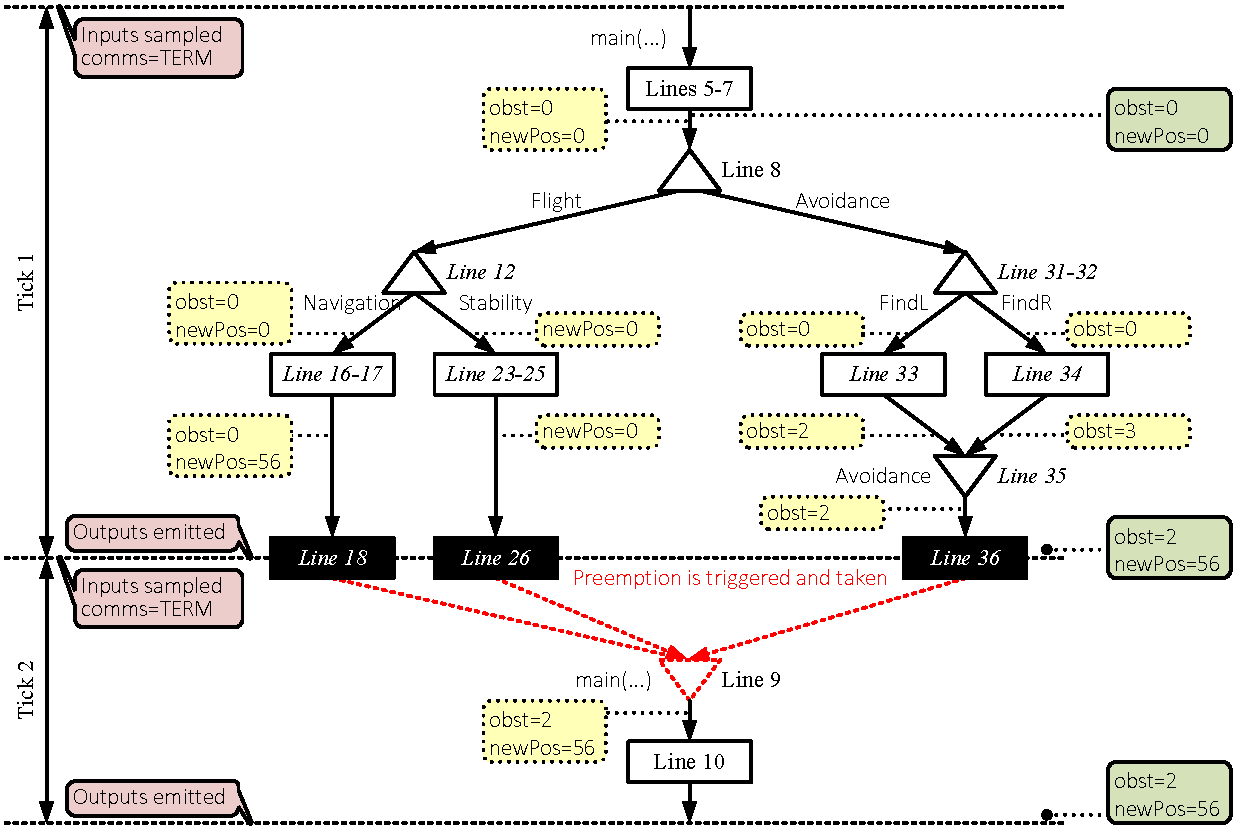
\includegraphics[width=\columnwidth]{images/uav_timing2.pdf}

	\caption{Possible execution trace of \texttt{UAV}.}
	\label{fig:forec_uav_timing2}
\end{figure}

\begin{figure}
	\centering
	
	\subfloat[Example code.] {
		\begin{minipage}[b]{0.8\textwidth}
			\lstinputlisting[style=full]{./code/abort.forec}
			\label{fig:forec_aborts_abort}
		\end{minipage}
	}

	\subfloat[Non-immediate and strong \texttt{abort}.] {
		\begin{tabular}{| p{0.4\textwidth} |}
			\hline
			Tick 1: \texttt{s} = \texttt{plus}(2,5,0) = 7.			\\ \hline
			Tick 2:	Preemption triggered and taken. ``7'' printed.	\\ 
			\hline
		\end{tabular}
		\label{fig:forec_aborts_strong}
	}
	\hspace{0.5cm}
	\subfloat[Non-immediate and weak \texttt{abort}.] {
		\begin{tabular}{| p{0.4\textwidth} |}
			\hline
			Tick 1: \texttt{s} = \texttt{plus}(2,5,0) = 7.			\\ \hline
			Tick 2:	Preemption triggered. 							\\
					\texttt{s} = \texttt{plus}(3,6,7) = 9.			\\
					Preemption taken. ``9'' printed.				\\ 
			\hline
		\end{tabular}
		\label{fig:forec_aborts_weak}
	}

	\subfloat[Immediate and strong \texttt{abort}.] {
		\begin{tabular}{| p{0.4\textwidth} |}
			\hline
			Tick 1: \texttt{s} = 1. Preemption triggered and taken.
					``1'' printed.									\\
			\hline
		\end{tabular}
		\label{fig:forec_aborts_immediate}
	}
	\hspace{0.5cm}
	\subfloat[Immediate and weak \texttt{abort}.] {
		\begin{tabular}{| p{0.4\textwidth} |}
			\hline
			Tick 1: \texttt{s} = 1. Preemption triggered.			\\
					Then \texttt{s} = \texttt{plus}(2,5,0) = 7.		\\
					Preemption taken. ``7'' printed.				\\
			\hline
		\end{tabular}
		\label{fig:forec_aborts_immediate_weak}
	}

	\caption{Abort variants.}
	\label{fig:forec_aborts}
\end{figure}

\subsection{Hierarchical Preemption}
The ``\verb$abort$~\emph{st} \verb$when$~(\expression{})''
statement provides preemption~\cite{timed_preemption}, which
is the termination of the \verb$abort$ body \emph{st} when
the condition \expression{} becomes true. The condition
\expression{} must be side-effect free. Preemption can be
used to model state machines succinctly. In Figure~\ref{fig:forec_uav_abort},
the \verb$main$ function of \verb$UAV$ has been extended to respond to 
external commands (\verb$comms$ line~\ref{code:forec_uav_abort_comms}). 
The \verb$abort$ statement 
on line~\ref{code:forec_uav_abort_abort} preempts the 
execution of all \verb$UAV$ tasks if the code \verb$TERM$ 
is received. The \verb$UAV$ descends safely and the program terminates 
(line~\ref{code:forec_uav_abort_descent}). 
A possible execution trace
of the extended \verb$UAV$ is given in Figure~\ref{fig:forec_uav_timing2}.
Line numbers in italic refer to Figure~\ref{fig:forec_uav}.
We now explain the semantics of the \verb$abort$ statement. 
The preemption of the \verb$abort$ must be triggered before it can be taken.
Preemption cannot be triggered when the \verb$abort$ body 
executes for the first time (e.g., tick 1 in Figure~\ref{fig:forec_uav_timing2}). 
For subsequent ticks, the
condition \expression{} is evaluated before the \verb$abort$
body can execute. Shared variables in \expression{} are
evaluated using their previous resynchronized value (\verb$pre$). If
\expression{} evaluates to true (a non-zero value following
the C convention), then the preemption is triggered and the
\verb$abort$ statement is terminated. At the start of tick 2
in Figure~\ref{fig:forec_uav_timing2}, preemption is triggered
because the condition evaluates to true. The \verb$abort$
statement also terminates if its body terminates normally. 

Like Esterel~\cite{timed_preemption}, the optional
\verb$weak$ and \verb$immediate$ keywords change the
temporal behavior of preemptions.
Figure~\ref{fig:forec_aborts_abort} is a short example containing
an \verb$abort$ with the optional keywords commented out.
Its execution is summarized in
Figure~\ref{fig:forec_aborts_strong}. The first tick ends with
threads \verb$main$, \verb$t0$, and \verb$t1$ modifying
their copies of \verb$s$ to 1, 2, and 5, respectively. Thus,
the resynchronized value of \verb$s$ is 7. At the start of
the second tick, the \verb$abort$'s preemption is triggered
and taken, resulting in ``7'' being printed. The \verb$weak$
keyword delays the \verb$abort$'s ability to take a triggered
preemption until its body cannot execute any further.
Uncommenting the \verb$weak$ keyword in Figure~\ref{fig:forec_aborts_abort} 
results in Figure~\ref{fig:forec_aborts_weak}. In the 
second tick, the triggered preemption is taken when
both threads complete their local tick (i.e., cannot execute
further). Thus, ``9'' is printed.

The \verb$immediate$ keyword allows preemption to be
triggered before the \verb$abort$ body can execute for the
first time. That is, the condition \expression{} is
evaluated immediately when execution first reaches the
\verb$abort$. Shared variables in \expression{}
are evaluated immediately using the thread's copies of shared variables, 
although their \verb$pre$ values are used for subsequent ticks. 
If \expression{} evaluates to true, then the
preemption is triggered. Uncommenting the \verb$immediate$ keyword 
in Figure~\ref{fig:forec_aborts_abort} results in 
Figure~\ref{fig:forec_aborts_immediate}. In the first 
tick, the preemption is triggered and taken before the 
\verb$abort$ body can execute. Thus,
``1'' is printed. Uncommenting both the \verb$weak$ and 
\verb$immediate$ keywords results in 
Figure~\ref{fig:forec_aborts_immediate_weak}.
In the first tick, the triggered preemption is 
taken only when both threads complete their local ticks. 
Hence, ``7'' is printed.

%For weak aborts, we choose not to check the preemption 
%after the abort body. This is because, if the preemption
%condition has shared variables, all the nested threads 
%would have to finish executing first before the values of
%the shared variables can be resolved to check the preemption
%condition. This would severely reduce the program's parallelism.
%In addition, for two nested weak abort statement with the
%same preemption condition, the outer condition can evaluate
%to a different value than the inner condition. The execution
%of code between the checking of the preemption conditions
%can change the state of the variables.

%If a statement should only be executed when an \verb$abort$ 
%has taken a preemption, then the 
%``\verb$weak$?~\verb$abort$~$st_0$~\verb$when immediate$?~(\expression{})~\verb$do$~$st_1$''
%variant should be used. The statement $st_1$ in the 
%``\verb$do$~$st_1$'' clause is only after a preemption is taken. 
%If the body terminates 
%normally, then $st_1$ is not executed. This allows
%$st_1$ to be used to implement \emph{cleanup} code.
%This \verb$abort-do$ variant can be structurally translated into an 
%ordinary \verb$abort$:
%\begin{lstlisting}[style=snippet]
%int preempted=0;
%weak? abort st(*$_1$*) when immediate? (preempted=exp);
%if (preempted) {st(*$_2$*);}
%\end{lstlisting}
%where \verb$preempted$ is a uniquely defined variable.

Many \verb$abort$ statements can be nested together to create 
a nesting (hierarchy) of preemptions.
As a direct consequence of the \verb$abort$ semantics, the
preemption behavior of an outer \verb$abort$ takes precedence 
over the inner \verb$abort$s. Figure~\ref{fig:forec_aborts_nested}
is a short example containing an immediate and weak
\verb$abort$ (line~\ref{code:forec_aborts_nested_outer}) 
with a nested immediate and strong \verb$abort$
(line~\ref{code:forec_aborts_nested_inner}).
In the first tick, preemption is triggered for the outer
weak \verb$abort$. The variable \verb$x$ is set to 2
and the inner strong \verb$abort$ preempts
immediately without executing its body. Next, \verb$x$ is set to 5 and the 
outer weak \verb$abort$ takes its preemption when 
it reaches the \verb$pause$ on line~\ref{code:forec_aborts_nested_pause}. 
Finally, ``5'' is printed.

\begin{figure}
	\centering

	\begin{minipage}[t]{0.75\columnwidth}
		\lstinputlisting[style=full]{./code/aborts_nested.forec}
	\end{minipage}

	\caption{Nesting of preemptions.}
	\label{fig:forec_aborts_nested}
\end{figure}


%-----------------------------------------------------------------------------

\subsection{Programming Safety-Critical Systems}
\label{sec:forecLanguage_programming}
The C language is popular for programming safety-critical embedded systems, 
but its semantics~\cite{programming_languages_c} includes unspecified 
and undefined behaviors~\cite{programming_languages_c_pitfalls}. Strict 
coding guidelines~\cite{safety_critical_coding_misrac_standard,safety_critical_coding_power_10,safety_critical_coding_jpl} 
are typically used by safety-critical programmers to help write well 
defined programs that are deterministic, understandable, maintainable, 
and straightforward to debug~\cite{wcet_software_structure,safety_critical_coding_misrac_overview}. 
The coding guidelines can be grouped into three main areas: 
\begin{itemize}
	\item Code clarity: These guidelines suggest a style for writing programs
		  free of ambiguous statements and to structure code for readability. 
		  For example, the use of indentation to clarify the nesting of 
		  \verb$if$-\verb$else$ statements.
		  Code clarity also helps static analyzers parse the program to 
		  attain greater analysis precision.
	\item Defensive programming: These guidelines help minimize the use of 
		  unspecified or undefined behaviors, which contribute towards
		  non-determinism. For example, expressions with side-effects should
		  not be used in function arguments. This is because the evaluation order of 
		  function arguments is unspecified.
	\item Runtime reliability: These guidelines help minimize runtime errors 
		  from occurring, even if the program is written correctly. 
		  For example, a runtime error occurs if a program requests for 
		  more memory than is available in the implemented system. 
\end{itemize}

ForeC forbids the use of unbounded recursion of function calls and 
thread forking to ensure runtime reliability. 
The synchrony hypothesis requires each tick to execute 
in finite time, which means all statements, except \verb$pause$, 
need to have bounded execution times. Unfortunately, loop constructs 
(\verb$for$ and \verb$while$) can have unbounded iterations, leading to
unbounded execution times. Thus, if a loop construct is used, 
then the programmer must guarantee that it always terminates or executes
a \verb$pause$ after a bounded number of iterations. Inspired by \pretc{}~\cite{pret_pretc}, 
we have extended the syntax of loops to help the programmer write 
bounded loops, shown in the first column of Table~\ref{table:forec_loop_translations}. 
The ``\verb$#n$'' after the loop header specifies 
that only up to \verb$n$ iterations can be executed.
The second column of Table~\ref{table:forec_loop_translations}
gives the structural translation of each bounded loop. 
For the translation of a bounded \verb$for$-loop,
the variable \verb$cnt$ tracks the number of iterations that have 
executed. The condition \verb$(cnt<n)$ guarantees that 
only up to \verb$n$ iterations are executed. The bounded 
\verb$while$-loop is translated into a bounded \verb$for$-loop. 
For the translation of a bounded \verb$do$-\verb$while$ loop, 
the variable \verb$first$ is used to delay the evaluation of 
\verb$cond$ to the second iteration. This delay emulates the 
execution behavior of a \verb$do$-\verb$while$ loop. 

\begin{table}
	\centering
	\renewcommand{\arraystretch}{1.25}
	
	\begin{tabular}{| l | l |}
		\hline
		\bf{Bounded Loop}						& \bf{Translation}											\\ 
		\hline
		\verb$for (init; cond; update) #n$		& \verb$int cnt=0;$											\\
		\verb${st}$								& \verb$for (init; cond && (cnt<n); (update,cnt++)) {st}$	\\ \hline
		\verb$while (cond) #n {st}$				& \verb$for (; cond;) #n {st}$								\\ \hline
		\verb$do {st} while (cond) #n$			& \verb$int first=1;$										\\
												& \verb$for (; cond && (first==0); first=0) #n {st}$		\\ \hline
	\end{tabular}
	
	\caption{The structural translations of bounded loops.}
	\label{table:forec_loop_translations}
\end{table}
